\begin{frame}
  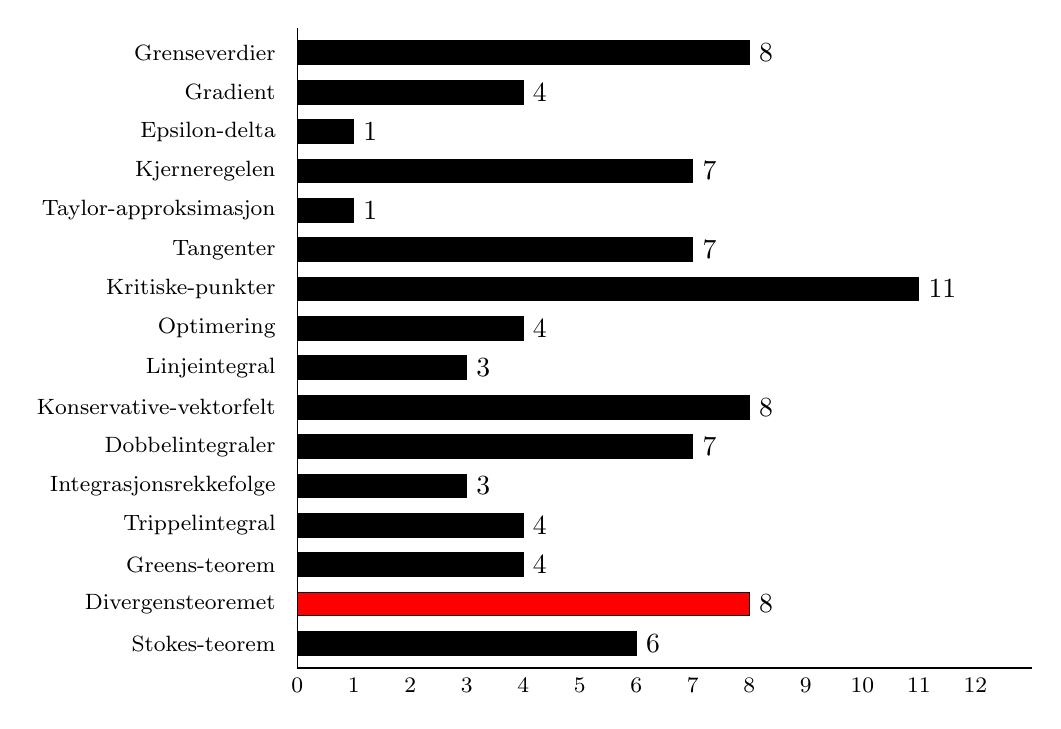
\begin{tikzpicture}
    \begin{axis}[ xbar=0pt, /pgf/bar shift=0pt, legend style={ legend columns=4,
        at={(xticklabel cs:0.5)}, anchor=north, draw=none }, ytick={0,...,15},
      ytick style={draw=none},% <- added
      axis y line*=none, axis x line*=bottom, tick label
      style={font=\footnotesize}, legend style={font=\footnotesize}, label
      style={font=\footnotesize}, xtick style={draw=none},% <- added
      xtick={0,1,...,12}, width=.9\textwidth, bar width=3mm, y dir = reverse,
      xmin=0, xmax=13, area legend,
      y=5mm, enlarge y limits={abs=0.625},
      style={text=black}, every axis plot/.append style={fill},
      nodes near coords, nodes near coords,
      yticklabels={%
        {\topicref{Grenseverdier}},
        {\topicref{Gradient}},
        {\topicref{Epsilon-delta}},
        {\topicref{Kjerneregelen}},
        {\topicref{Taylor-approksimasjon}},
        {\topicref{Tangenter}},
        {\topicref{Kritiske-punkter}},
        {\topicref{Optimering}},
        {\topicref{Linjeintegral}},
        {\topicref{Konservative-vektorfelt}},
        {\topicref{Dobbelintegraler}},
        {\topicref{Integrasjonsrekkefolge}},
        {\topicref{Trippelintegral}},
        {\topicref{Greens-teorem}},
        {\topicref{Divergensteoremet}},
        {\topicref{Stokes-teorem}}}]
      \addplot[fill=black] coordinates {(8,0)};
      \addplot[fill=black] coordinates {(4,1)};
      \addplot[fill=black] coordinates {(1,2)};
      \addplot[fill=black] coordinates {(7,3)};
      \addplot[fill=black] coordinates {(1,4)};
      \addplot[fill=black] coordinates {(7,5)};
      \addplot[fill=black] coordinates {(11,6)};
      \addplot[fill=black] coordinates {(4,7)};
      \addplot[fill=black] coordinates {(3,8)};
      \addplot[fill=black] coordinates {(8,9)};
      \addplot[fill=black] coordinates {(7,10)};
      \addplot[fill=black] coordinates {(3,11)};
      \addplot[fill=black] coordinates {(4,12)};
      \addplot[fill=black] coordinates {(4,13)};
      \addplot[fill=red] coordinates {(8,14)};
      \addplot[fill=black] coordinates {(6,15)};
    \end{axis}
  \end{tikzpicture}
\end{frame}

\begin{frame}
  \subsection{Divergensteoremet}\label{subsec:Divergensteoremet}
  \frametitle{Divergensteoremet}
    \centerline{%
    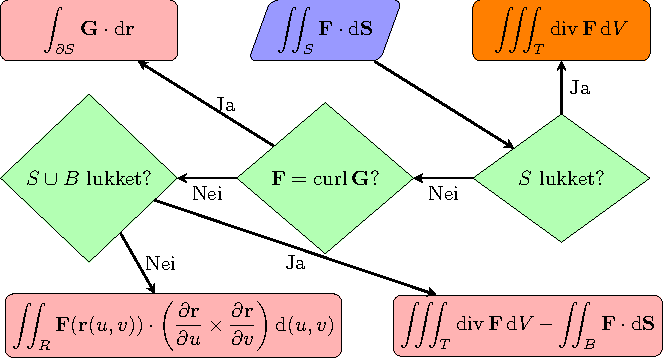
\includegraphics{../img/flytskjema-overflateintegral-1}
  }
\end{frame}

\begin{frame}
  \begin{theorem}[Divergensteoremet]
    La $V$ være et lukket volum i rommet som har en parametriserbar overflate
    $S$, og la enhetsnormalen $\vek{n}$ peke ut av $V$. Dersom $\F$ er et
    vektorfelt som har kontinuerlige partiellderiverte på $V$ da er
    %
    \begin{equation*}
      \iint_S \F \cdot \vek{n} \dS = \iiint_V \div \F \dV
    \end{equation*}
  \end{theorem}
  \begin{minipage}{.45\textwidth}
    \begin{intuisjon}
      % 
      Anta du har en \emph{full} bolle med vann, og heller på mer vann. Hva
      skjer? Jo det renner vann ut av overflaten til bollen. Med andre ord er
      summen av endring i vesketetthet ($\iiint_V \div \F \dV$) lik
      hvor mye væske som forlater overflaten ($\iint_S \F \cdot \dSS$).
      % 
    \end{intuisjon}
\end{minipage}
\begin{minipage}{.45\textwidth}
  \centering
    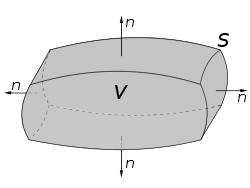
\includegraphics[scale=0.75]{../img/bolle2.png}
  \end{minipage}
\end{frame}

\begin{frame}
  \begin{oppgave}{V2012, Oppgave 5} Finn fluksen av vektorfeltet $F(x, y, z) =
    (\sin y) 2 \I + x\J + \only<1-5>{x}\only<6>{3}z\K$ inn i enhetskula med sentrum i origo.
  \end{oppgave}
  \visible<2->{
  \textbf{To krav:}
  \begin{enumerate}
      \item Er flaten $V$ avgrenset av randen $S$ lukket og
      enkeltsammenhengende?
      Ja, enhetskula er åpenbart lukket og enkeltsammenhengdende.
      \item Har vektor feltet $F$ kontinuerlige partiellderiverte definert på
      $W$. Ja, alle polynomer og $\sin x$ er deriverbare. 
  \end{enumerate}}\only<3->{
  Har at normalvektoren er $-\vek{n}$ siden den skulle peke \emph{inn} i kula.
  \begin{align*}
    \iint_{S} \F \cdot (-\vek{n}) \dS
    & = -\iint_{S} \F \cdot \vek{n}\dS
    \overset{\text{Gauss}}{=} -\iiint_{V} \div \F \dV \\
    & = -\iiint_V 0 + 0 + \only<1-5>{x}\only<6>{3} \dV 
      = -\iiint_V \only<1-5>{x}\only<6>{3} \dV\only<5>{=0}\only<6>{=\,?}
  \end{align*}}
\end{frame}

\begin{frame}
  \frametitle{Divergensteoremet}
    \centerline{%
    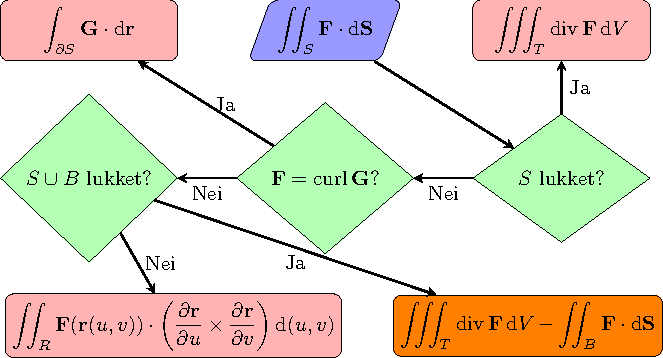
\includegraphics{../img/flytskjema-overflateintegral-4}
  }
\end{frame}


\begin{frame}
    \begin{example}
        Halvkulen $T$ er bestemt av 
        %
        $x^2 + y^2 + z^2 \leq 1$ og $z \geq 0$
        %
        Vi lar $S$ betegne den krumme delen av overflaten til $T$. 
        Vektorfeltet $\mathbf{F}$ er gitt ved 
        %
        \begin{equation*}
            \mathbf{F}(x,y,z)
            = x(z+z^2)\I - (yz^2 + xe^y)\J + (xze^y + 1)\K
        \end{equation*}
        %
        Bestem fluksintegralet 
        %
        $ \displaystyle
        \iint_{S} \mathbf{F} \cdot \vek{n} \, \mathrm{d}S
        $
        %
        der $\vek{n}$ har positiv $z$-komponent. 
      \end{example}
      \begin{enumerate}
        \item Regne ut $\text{div } \mathbf{F} \only<2->{=(z + z^2)-(z^2 + xe^y)
          + xe^y} \only<3->{=z}$
      \end{enumerate}
      \only<1-2>{
      \begin{equation*}
        \div \F 
        = \diffp{}{x}\bigl( x(z+z^2) \bigr) - \diffp{}{y}\bigl( yz^2 + xe^y \bigr) + \diffp{}{z}\bigl( xze^y + 1 \bigr)
      \end{equation*}}
      \begin{enumerate}\setcounter{enumi}{1}
        \item Bruke divergensteoremet på hele overflaten til $T$
      \end{enumerate}
      \only<3->{
        \begin{equation*}
          \iint_{T} \F \cdot \vek \dS
          \overset{\text{Gauss}}{=} \iiint_V \only<3>{\div \F}\only<4->{z} \dV
          \only<5>{= \int_0^{\pi/2}\int_0^{2\pi}\int_0^1 \rho \cos \varphi (\rho^2
          \sin \varphi )\dd \rho \dd \varphi \dT}
          \only<6>{= 2\pi \left[ \frac{\rho^4}{4} \right]_0^1 \left[ -\frac{(\cos \varphi)^2}{2} \right]_0^{\pi/2}}
          \only<7>{= 2\pi \left[  \frac{1}{4} - 0 \right]\left[  \frac{1^2}{2} - 0\right]= \frac{\pi}{4}}
        \end{equation*}
      }
      \begin{enumerate}\setcounter{enumi}{2}
        \item Finne fluksen ut av $S$.
    \end{enumerate}

\end{frame}

\begin{frame}
%\begin{frame}{Pixelweise Segmentierung}
    \begin{figure}[ht]
        \begin{minipage}[b]{0.30\linewidth}
            \centering
            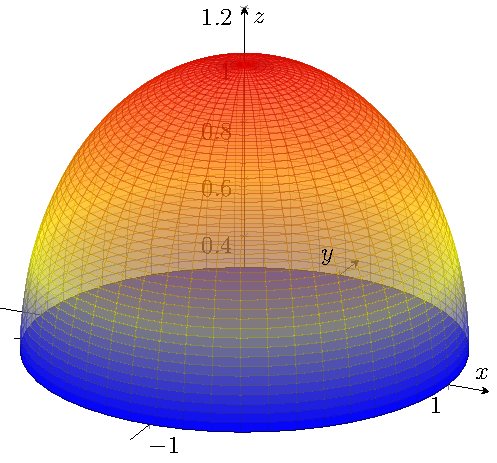
\includegraphics[width=\textwidth]{../img/3-Lukket.pdf}
%            \caption*{$\iint_{D} F \cdot \hat{N} \mathrm{d}S$}
        \end{minipage}
        \hspace{0.30cm}
        \begin{minipage}[b]{0.30\linewidth}
            \centering
            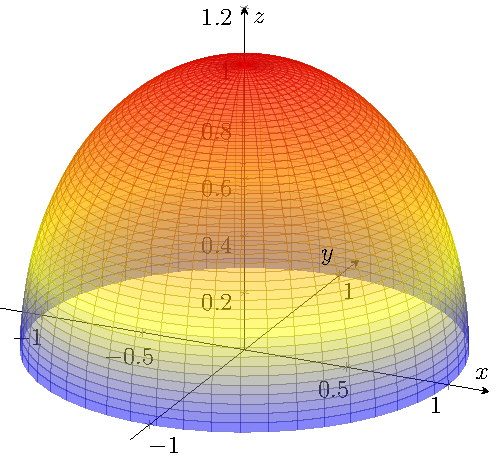
\includegraphics[width=\textwidth]{../img/1-Topp.pdf}
%            \caption*{$\iint_{S} F \cdot \hat{N} \mathrm{d}S$}
        \end{minipage}
        \hspace{0.30cm}
        \begin{minipage}[b]{0.30\linewidth}
            \centering
            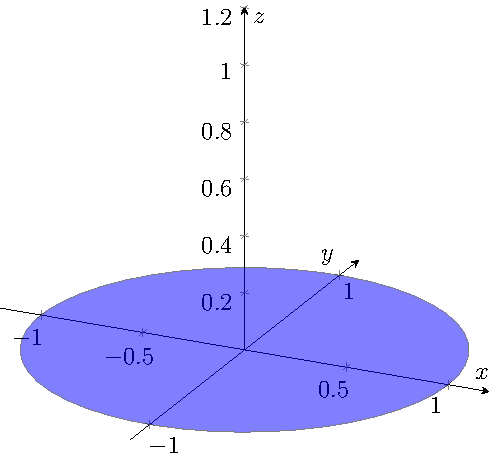
\includegraphics[width=\textwidth]{../img/2-Bunn.pdf}
%            \caption*{$\iint_{B} F \cdot \hat{N} \mathrm{d}S$}
        \end{minipage}
    \end{figure}
\begin{align*}
    \iint_{T} \F \cdot \vek{n} \dS
    \qquad =  \qquad 
    \iint_{S} \F \cdot \vek{n} \dS
    \qquad + \qquad  
    \iint_{B} \F \cdot \vek{n} \dS
\end{align*}
\end{frame}

\begin{frame}
%\begin{frame}{Pixelweise Segmentierung}
    \begin{figure}[ht]
        \begin{minipage}[b]{0.30\linewidth}
            \centering
            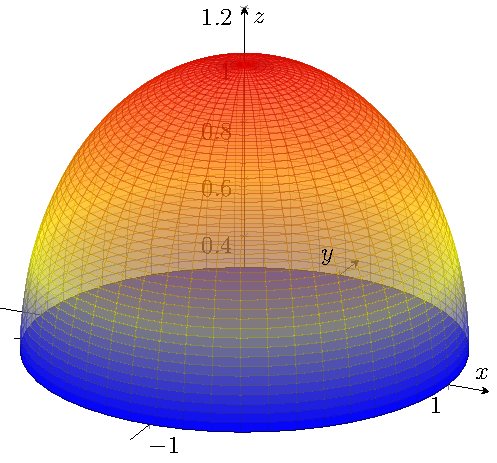
\includegraphics[width=\textwidth]{../img/3-Lukket.pdf}
%            \caption*{$\iint_{D} F \cdot \hat{N} \mathrm{d}S$}
        \end{minipage}
        \hspace{0.30cm}
        \begin{minipage}[b]{0.30\linewidth}
            \centering
            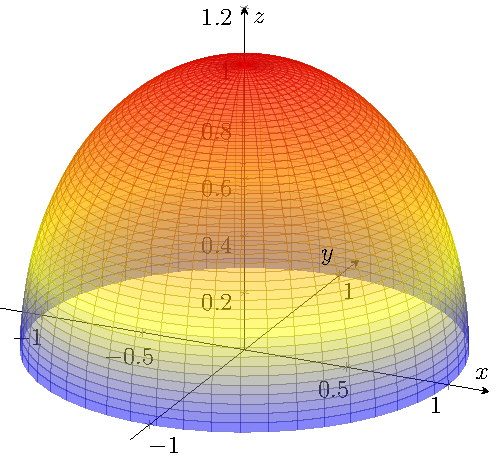
\includegraphics[width=\textwidth]{../img/1-Topp.pdf}
%            \caption*{$\iint_{S} F \cdot \hat{N} \mathrm{d}S$}
        \end{minipage}
        \hspace{0.30cm}
        \begin{minipage}[b]{0.30\linewidth}
            \centering
            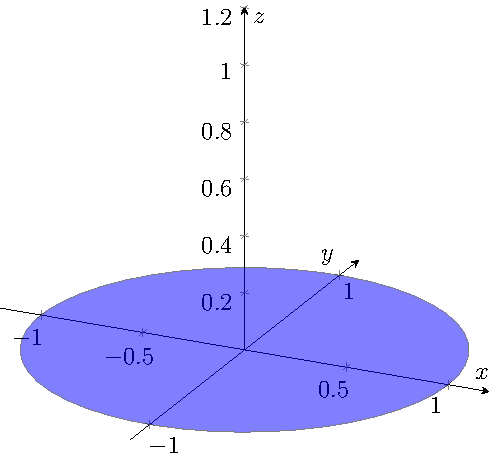
\includegraphics[width=\textwidth]{../img/2-Bunn.pdf}
%            \caption*{$\iint_{B} F \cdot \hat{N} \mathrm{d}S$}
        \end{minipage}
    \end{figure}
\begin{align*}
    \iiint_{T} \text{div }\F \dV
    \qquad =  \qquad 
    \iint_{S} \F \cdot \vek{n} \dS
    \qquad + \qquad  
    \iint_{B} \F \cdot \vek{n} \dS
\end{align*}
\end{frame}

\begin{frame}
%\begin{frame}{Pixelweise Segmentierung}
    \begin{figure}[ht]
        \begin{minipage}[b]{0.30\linewidth}
            \centering
            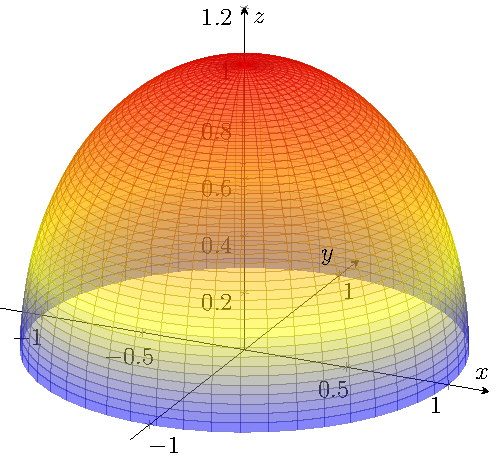
\includegraphics[width=\textwidth]{../img/1-Topp.pdf}
%            \caption*{$\iint_{D} F \cdot \hat{N} \mathrm{d}S$}
        \end{minipage}
        \hspace{0.30cm}
        \begin{minipage}[b]{0.30\linewidth}
            \centering
            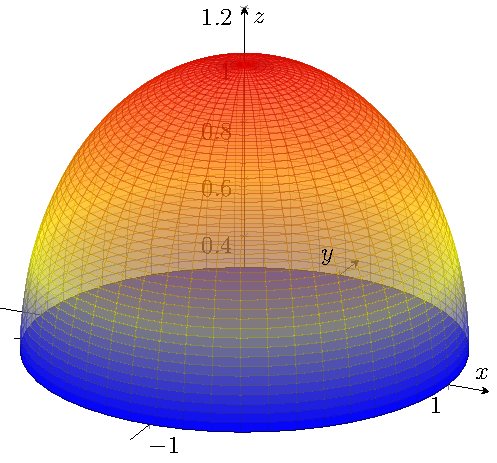
\includegraphics[width=\textwidth]{../img/3-Lukket.pdf}
%            \caption*{$\iint_{S} F \cdot \hat{N} \mathrm{d}S$}
        \end{minipage}
        \hspace{0.30cm}
        \begin{minipage}[b]{0.30\linewidth}
            \centering
            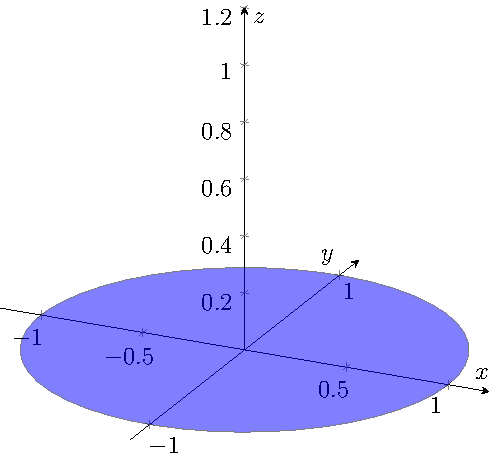
\includegraphics[width=\textwidth]{../img/2-Bunn.pdf}
%            \caption*{$\iint_{B} F \cdot \hat{N} \mathrm{d}S$}
        \end{minipage}
    \end{figure}
\begin{align*}
    \iint_{S} \F \cdot \vek{n} \dS
    \qquad =  \qquad 
    \iiint_{T} \div \F \dV 
    \qquad - \qquad  
    \iint_{B} \F \cdot \vek{n} \dS
\end{align*}
\end{frame}


\begin{frame}
  Reminder:
  $
    \mathbf{F}(x,y,z)
    = x(z+z^2)\I - (yz^2 + xe^y)\J + (xze^y + 1)\K
    $ \\ \medskip
    
    Beregner overflateintegralet \emph{ut} av bunnen. Siden normalvektoren må peke ut av flaten får vi $\vek{n} = (0,0,-1)$ Så 
    %
    \begin{align*}
        \iint_{B} \F \cdot \vek{n} \dS
        & =  \iint_{B} \F \cdot (0,0-1)\dS  \\
        & = -\iint_{B} (x \cdot \only<2->{\textcolor{red}{0}}\only<1>{\textcolor{red}{z}} \cdot e^{y} + 1) \dS \visible<2->{
        = -\iint_{B} 1 \dS
        = - \pi}
    \end{align*}\visible<3->{
    Siden $z = 0$ og $B$ er en sirkel med radius $1$. Oppsumert har vi altså
\begin{align*}
    \iint_{S} \F \cdot \vek{n} \dS
    & = 
    \iiint_{T} \div \F \dV
    -
    \iint_{B} \F \cdot \vek{n} \dS \\
    & = \frac{\pi}{4} \qquad \qquad \ \: \ - \qquad(-\pi) \\
    & = \frac{5\pi}{4}
\end{align*}}
\end{frame}

%%% Local Variables:
%%% mode: latex
%%% TeX-master: "main"
%%% End:
